\section{核心星云指数}
\begin{frame}
	核心星云指数用于衡量一段时间内用户对整个经济体的贡献。精确的计算这一指标是十分困难的,
  因此,我们使用了一个近似算法。在该近似算法中,我们考虑了两个重要的因素, 即账户持有的币龄及账户在交易网络中的位置信息。

  我们使用一段时间内的链上的交易记录作为核心星云指数的数据来源:
  \begin{align}
  \Theta(t_0) = \{(s, t, w, \tau)\ |\ t_0 - T \le \tau \le t_0\ \land \ a > 0 \land s \neq t \}
  \end{align}
  \noindent 基于$\Theta(t_0)$,我们可以构造有向加权图,其中节点为账户地址,一个交易为从节点$s$到节点$d$的有向边,
  边的权值的$w$,边的时间为$\tau$。
  对于账户$a \in \mathcal{A}$,其核心星云指数$\mathcal{C}(a)$的计算基于$\Theta(t_0)$,即
  \begin{align}
  \mathcal{C}(a) = \Omega(\beta(a)) \times{} \Psi(\gamma(a))
  \label{eq:rank}
  \end{align}
  \noindent 其中$\beta(a)$为一段时间内账户$a$持有的资产的数量的中值;$\gamma(a)$为账户$a$在一段时间内的出入度指标。
\end{frame}

\begin{frame}
\frametitle{资产中值$\beta(a)$}
对于时间段$[t_0\ −\ T,\ t_0]$,区块链系统中存在$n$个区块,记为
\[
B_0, B_1, \dots, B_n
\]
\noindent 其中$B_{i}$ 为$B_{i+1}$的父块。对于账户$a \in \mathcal{A}$,其在每个区块结束后,
其相应的账户余额为
\[
d^a_0, d^a_1, \dots, d^a_n
\]
上述序列按从小到大排序后可以得到
\[
d^a_{(0)}, d^a_{(1)}, \dots, d^a_{(n)}
\]
其中$d^a_{(i)} < d^a_{(i+1)}, 0\le i \le {n-1}$,由此,可以得到
\begin{align}
\beta(a) = \left\{ \begin{array}{rcl}
{d^a_{(k)}} & \mbox{for} & n=2\times{}k, k=1, 2, 3, \ldots \\
{(d^a_{(k)} + d^a_{(k+1)})/2} & \mbox{for} & n=2\times{}k + 1, k=1, 2, 3, \ldots
\end{array}\right.
\end{align}
资产中值一定程度上代表了“币龄”,即账户中需要至少持有该资产一半以上的时间。
\end{frame}

\begin{frame}
\frametitle{出入度指标$\gamma$}
出入度指标的计算首先需要对交易图进行“去交易环”处理。交易环(forwarding loop)是指一组按时间顺序进行的交易行程的环路。
一个交易环在节点$v$开始并结束,是交易图中边的集合,记为$H(v)$,即,
\[\begin{split}
H(v) =& \{(v, v_1, w_1, \tau_1), (v_1, v_2, w_2, \tau_2), \dots, (v_i, v_{i+1}, w_{i}, \tau_i), \\
& \dots, (v_n, v, w_{n+1}, \tau_{n+1})\}
\end{split}\]
\noindent 其中,$\forall 1\le i \le {n-1} : \tau_i \le \tau_{i+1} $。
\end{frame}

\begin{frame}
\frametitle{出入度指标$\gamma$}
\begin{figure}
\centering
  \begin{tikzpicture}
\pgfmathsetmacro{\XTD}{3.8}
\pgfmathsetmacro{\XMD}{1.2}
\pgfmathsetmacro{\YTD}{3.8}


\tikzset{
  node/.style={draw, circle, on grid, align=center, minimum height=2ex},
  thread/.style={draw, rectangle, on grid, align=center,color=gray!30,
  fill=gray!30,
  rounded corners,
  minimum height=3ex,fit=#1},
}

\node[node] (v) at (0, 0) {$v$};
\node[node] (v1) at (0, \YTD) {$v_1$};
\node[node] (v2) at (\XTD, \YTD) {$v_2$};
\node[node] (v3) at (\XTD, 0) {$v_3$};

\draw[->,>=stealth'] (v) to [out=135, in=225] node[left, midway] {$w=100$,$\tau=1$} (v1);
\draw[->,>=stealth'] (v1) to [out=45, in=135] node[above, midway] {$w=10$,$\tau=2$} (v2);
\draw[->,>=stealth'] (v1) to [out=315, in=225] node[below, midway] {$w=100$,$\tau=5$} (v2);
\draw[->,>=stealth'] (v2) to [out=315, in=45] node[right, midway] {$w=10$,$\tau=3$} (v3);
\draw[->,>=stealth'] (v3) to [out=225, in=315] node[below, midway] {$w=10$,$\tau=4$} (v);

\node at (2.5*\XTD, 0.5*\YTD) {
$\begin{aligned}
     H(v) = \{&(v, v1, 100, 1),\\
     &(v1, v2, 10, 2), \\
     &(v2, v3, 10, 3), \\
     &(v3, v, 10, 4) \}
  \end{aligned}$};
\end{tikzpicture}

\caption{loop\label{fig:loop}}
\end{figure}

\end{frame}

\begin{frame}
\frametitle{出入度指标$\gamma$}
在找到交易环后,需要进行去交易环处理。假设系统中存在$n$个交易环,按照交易环在交易图中出现的顺序记为
\[
H^1(v_1), H^2(v_2), \dots, H^n(v_n)\]
\noindent 其中,$H^i(v_i)$中交易金额最小的交易为 $(s^i_m, t^i_m, w^i_m, \tau^i_m)$,即
\[
\forall (s^i, t^i, w^i, \tau^i) \in \mathcal{T} : w^i \ge w^i_m
\]
\noindent 然后,需要依次将$H^i(v_i)$中所有的交易减去相应的最小交易量$w^i_m$,
如果新的交易量为0,则移除该交易,即
\[
\mathcal{E}((s, t, w, \tau), w_m) = \left\{ \begin{array}{rcl}
(s, t, w-w_m, \tau) & \mbox{if} & w \ne w_m \\
\phi & \mbox{if} & w = w_m
\end{array}\right.
\]
\begin{align}
\Theta^{\prime}(t_0)=\Theta(t_0)-H^i(v) \cup \{\mathcal{E}(t), t\in H^i(v_i)\} \quad i = 1, 2,\dots, n
\end{align}
\end{frame}

\begin{frame}
\frametitle{出入度指标$\gamma$}
\begin{figure}
\centering
\begin{tikzpicture}
\pgfmathsetmacro{\XTD}{3.8}
\pgfmathsetmacro{\XMD}{1.2}
\pgfmathsetmacro{\YTD}{3.8}


\tikzset{
  node/.style={draw, circle, on grid, align=center, minimum height=2ex},
  thread/.style={draw, rectangle, on grid, align=center,color=gray!30,
  fill=gray!30,
  rounded corners,
  minimum height=3ex,fit=#1},
}

\node[node] (v) at (0, 0) {$v$};
\node[node] (v1) at (0, \YTD) {$v_1$};
\node[node] (v2) at (\XTD, \YTD) {$v_2$};
\node[node] (v3) at (\XTD, 0) {$v_3$};
\draw[->,>=stealth'] (v) to [out=135, in=225] node[left, midway] {$w=90$,$\tau=1$} (v1);
\draw[->,>=stealth'] (v1) to [out=315, in=225] node[below, midway] {$w=100$,$\tau=5$} (v2);

\end{tikzpicture}
\caption{\reffig{fig:loop}去掉交易环后的交易图 \label{fig:no-loop}}
\end{figure}

\end{frame}

\begin{frame}
\frametitle{出入度指标$\gamma$}
记节点$v$的转入金额为$p(v)$,则
\begin{align}
p(v) = \sum_{(s_i, v, w_i, \tau_i) \in \Theta^{\prime}(t_0)}{w_i}
\end{align}
\noindent 同理,节点$v$的转出金额有
\begin{align}
q(v) = \sum_{(v, t_i, w_i, \tau_i) \in \Theta^{\prime}(t_0)}{w_i}
\end{align}
\noindent 由此,
对于节点$v$,其出入度指标$\gamma(v)$为

\begin{align}
\mathcal{G}(v) = (p(v) + q(v)) \cdot e^{-2\sin^2{(\frac{\pi}{4} - \arctan\frac{q(v)}{p(v)})}}
\end{align}

\begin{align}
\gamma(v) = (\frac{\theta\cdot \mathcal{G}(v)}{\mathcal{G}(v) + \mu})^{\lambda}
\end{align}
\end{frame}

\begin{frame}
\frametitle{出入度指标$\gamma$}
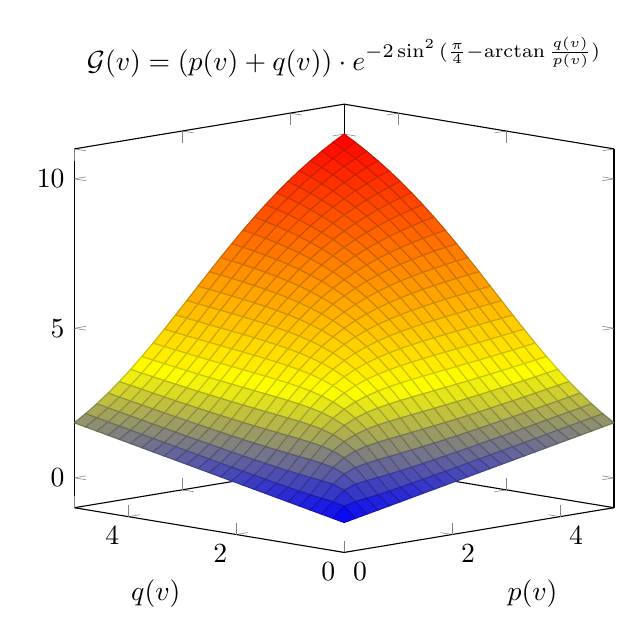
\begin{tikzpicture}[
    declare function={tf(\x)=(pi/4-rad(atan(\x)));},
    declare function={func(\x,\y)=sin(tf(\y/\x)*180/pi);}
]
\begin{axis}[
    view={315}{10},
    title={$
\mathcal{G}(v) = (p(v) + q(v)) \cdot e^{-2\sin^2{(\frac{\pi}{4} -
\arctan\frac{q(v)}{p(v)})}}$},
    xlabel=$p(v)$,
    ylabel=$q(v)$,
]

\addplot3 [
        surf,
        domain=0:5,
        domain y=0:5,
    ] {(x+y)*exp((-2)*(func(x,y))^2)};
\end{axis}
\end{tikzpicture}

\end{frame}



\begin{frame}
\frametitle{Wilbur函数}
%考虑到不同的使用场景及不同的性质,星云指数的计算是十分复杂的,然而,我们可以总结出一般意义上的星云指数计算函数的性质。

我们记星云指数的计算函数为\(f(x)\),其中\(x\)
为星云指数需要参考的因素,可以为持有的余额、币龄或账户的出入度。$f(x)$需要满足两个性质,

\begin{property}
对于任意大于$0$的两个输入变量$a$,$b$,其计算函数之和小于其和的计算函数。
%对于任意输入$x$,将其拆分后的计算函数之和小于原计算函数。
\end{property}

\begin{align}
f(a+b)>f(a)+f(b) \quad a>0,b>0
\end{align}

\begin{property}
当任意大于$0$的两个输入变量趋近于无穷大时,其计算函数之和趋近于其和的计算函数。
\end{property}

\begin{align}
\lim\limits_{a \to \infty, b\to \infty} f(a+b) = f(a) + f(b)\quad a>0, b>0
\end{align}

\end{frame}

\begin{frame}
\frametitle{Wilbur函数}
\noindent 满足上述两个性质的函数有很多,在此,我们仅给出一个满足上述性质的函数,该函数的图形如\reffig{fig-nr}所示。
\begin{align}
f(x) = x/(1 + e^{a + b\cdot x}) \quad a>1,b<0
\end{align}

\begin{figure}
\centering
\begin{tikzpicture}[
    scale=0.8,
    declare function={func(\x,\mu) = (\x / (1 + exp(\mu-\x)));},
    declare function={linefunc(\x) = \x;}
]
\begin{axis}[
    axis lines=left,
    enlargelimits=upper,
ticks=none,axis x line=bottom,axis y line=left,xlabel={Nebulas Rank Factor},
  ylabel={星云指数},
      legend pos=north west
]
\addplot [dotted, domain=0:10, blue] {linefunc(x)};
\addplot [smooth, domain=0:10, red] {func(x,3)};
\addlegendentry{$f(x)=x$}
\addlegendentry{$f(x)=x/(1 + e^{a + b\cdot x})$}
\end{axis}
\end{tikzpicture}
\caption{星云指数计算函数曲线 \label{fig-nr}}
\end{figure}
\end{frame}

\begin{frame}
\frametitle{核心星云指数验证}

为了验证该函数的有效性,我们根据以太坊中的数据,计算了以太坊中地址的星云指数,并根据其市值变化计算了两者的相关性。
%测试数据包括了以太坊从2017年5月1日起至2017年6月30日(3629091区块至3955158区块)的所有交易记录,以及ETH日均价格(对美元)和日均总交易量~\cite{coinmarketcap}。


\reffig{fig-eth-simu}表示了以太坊的市值与星云指数随时间变化趋势,如图所示,星云指数能够有效反映以太坊市值变化,二者的相关系数(Correlation coefficient)为0.84427,$p$值(p-value)为$4.48\times{}10^{-17}<0.001$。
%说明函数~\ref{eq:rank}能够有效表示用户对整个经济体的贡献。


\begin{figure}
\centering
\begin{tikzpicture}[scale=0.8]
  \begin{axis}[
  axis y line*=left,
  axis x line=none,
%ticks=none,
ylabel={以太坊市值(美元)},
%xtick={0,10,20,30,40,50,60},
%xlabel={时间(天)}
    ]
\addplot[smooth, mark=., color=red] table [x=day, y=nr, col sep=comma] {eth_simu.csv};
\label{plot_one}

\end{axis}
  \begin{axis}[
%ticks=none,
legend pos=north west,
%ylabel={星云指数},
xlabel={时间(天)},
xtick={0,10,20,30,40,50,60},
ytick={1,2},
axis y line*=right
    ]
    \addlegendimage{/pgfplots/refstyle=plot_one}\addlegendentry{星云指数}

    \addplot[smooth, mark=x] table [x=day, y=cap, col sep=comma] {eth_simu.csv};
    \label{plot_two}
      \addlegendentry{以太坊市值}
\end{axis}

\end{tikzpicture}
\caption{以太坊之上的星云指数及以太坊市值}
\label{fig-eth-simu}
\end{figure}
\end{frame}
